% The Three Leaks: report. Every number comes from numbers.tex, written by the pipeline (make report).
\documentclass[11pt]{article}
\pdfgentounicode=1
\usepackage[T1]{fontenc}
\usepackage[utf8]{inputenc}
\input{glyphtounicode}
\usepackage{XCharter}
\usepackage[scaled=0.92]{sourcesans}
\usepackage[a4paper,margin=1in]{geometry}
\usepackage{microtype}
\usepackage{amsmath}
\usepackage{graphicx}
\usepackage{booktabs}
\usepackage{xcolor}
\usepackage{titlesec}
\usepackage{enumitem}
\usepackage{caption}
\usepackage{float}
\usepackage[hidelinks]{hyperref}
\definecolor{accent}{HTML}{1F3A5F}
\definecolor{soft}{HTML}{EEF1F5}
\titleformat{\section}{\sffamily\color{accent}\large\bfseries}{\thesection}{0.6em}{}
\titleformat{\subsection}{\sffamily\color{accent}\bfseries}{\thesubsection}{0.6em}{}
\captionsetup{font=small,labelfont={bf,sf}}
\setlist{itemsep=2pt,topsep=3pt}
\graphicspath{{../results/figures/}}
% Written by threeleaks.numbers from results/numbers.json. Do not edit by hand.
\newcommand{\CalibMidcapOneFiveZeroAlpha}{2.9\%}
\newcommand{\CalibMidcapOneFiveZeroMonths}{58}
\newcommand{\CalibMidcapOneFiveZeroT}{1.20}
\newcommand{\CalibNextFiveZeroAlpha}{-0.29\%}
\newcommand{\CalibNextFiveZeroMonths}{186}
\newcommand{\CalibNextFiveZeroT}{-0.17}
\newcommand{\CalibNiftyFiveZeroAlpha}{0.78\%}
\newcommand{\CalibNiftyFiveZeroMonths}{236}
\newcommand{\CalibNiftyFiveZeroT}{0.58}
\newcommand{\CalibSensexAlpha}{1.1\%}
\newcommand{\CalibSensexMonths}{236}
\newcommand{\CalibSensexT}{0.76}
\newcommand{\CalibSmallcapTwoFiveZeroAlpha}{-3.33\%}
\newcommand{\CalibSmallcapTwoFiveZeroMonths}{62}
\newcommand{\CalibSmallcapTwoFiveZeroT}{-1.42}
\newcommand{\CardCommissionMedian}{1.24\%}
\newcommand{\CardCommissionPNineZero}{1.64\%}
\newcommand{\CardFunds}{521}
\newcommand{\CardLuck}{89}
\newcommand{\CardSector}{221}
\newcommand{\CardShort}{57}
\newcommand{\CardSkill}{154}
\newcommand{\CardUnder}{0}
\newcommand{\ClosetAfterControlN}{33}
\newcommand{\ClosetAfterControlTeBefore}{11.5\%}
\newcommand{\ClosetAfterControlTePost}{11.4\%}
\newcommand{\ClosetAfterDidP}{0.166}
\newcommand{\ClosetAfterDidRTwo}{-0.33}
\newcommand{\ClosetAfterDidTe}{0.8\%}
\newcommand{\ClosetAfterLargeN}{27}
\newcommand{\ClosetAfterLargeRTwoBefore}{0.88}
\newcommand{\ClosetAfterLargeRTwoPost}{0.97}
\newcommand{\ClosetAfterLargeTeBefore}{4.05\%}
\newcommand{\ClosetAfterLargeTePost}{4.72\%}
\newcommand{\ClosetLaterControlN}{29}
\newcommand{\ClosetLaterControlTeBefore}{11.5\%}
\newcommand{\ClosetLaterControlTePost}{9.82\%}
\newcommand{\ClosetLaterDidP}{0.050}
\newcommand{\ClosetLaterDidRTwo}{-0.06}
\newcommand{\ClosetLaterDidTe}{1.04\%}
\newcommand{\ClosetLaterLargeN}{22}
\newcommand{\ClosetLaterLargeRTwoBefore}{0.89}
\newcommand{\ClosetLaterLargeRTwoPost}{0.93}
\newcommand{\ClosetLaterLargeTeBefore}{3.84\%}
\newcommand{\ClosetLaterLargeTePost}{3.22\%}
\newcommand{\CommissionGapMean}{1.18\%}
\newcommand{\CommissionGapMedian}{1.2\%}
\newcommand{\CommissionGapPTwoFive}{0.9\%}
\newcommand{\CommissionGapPSevenFive}{1.5\%}
\newcommand{\CommissionPairs}{622}
\newcommand{\CommissionPlaceboTwoZeroOneSixChange}{0.05\%}
\newcommand{\CommissionPlaceboTwoZeroOneSixP}{0.018}
\newcommand{\CommissionPlaceboTwoZeroTwoTwoChange}{-0.01\%}
\newcommand{\CommissionPlaceboTwoZeroTwoTwoP}{0.334}
\newcommand{\CommissionSharePositive}{100.0\%}
\newcommand{\CommissionTerAfter}{0.96\%}
\newcommand{\CommissionTerBefore}{1.07\%}
\newcommand{\CommissionTerChange}{-0.11\%}
\newcommand{\CommissionTerP}{<0.001}
\newcommand{\CommissionTerPWilcoxon}{<0.001}
\newcommand{\CommissionTerPairs}{266}
\newcommand{\CommissionTerShareNarrowed}{66.9\%}
\newcommand{\CommissionUpfrontChange}{-0.12\%}
\newcommand{\CommissionUpfrontP}{<0.001}
\newcommand{\CommissionWilcoxonP}{<0.001}
\newcommand{\CommissionYearTwoZeroOneThreeMedian}{0.57\%}
\newcommand{\CommissionYearTwoZeroOneFourMedian}{0.69\%}
\newcommand{\CommissionYearTwoZeroOneFiveMedian}{0.77\%}
\newcommand{\CommissionYearTwoZeroOneSixMedian}{0.86\%}
\newcommand{\CommissionYearTwoZeroOneSevenMedian}{0.99\%}
\newcommand{\CommissionYearTwoZeroOneEightMedian}{1.04\%}
\newcommand{\CommissionYearTwoZeroOneNineMedian}{0.97\%}
\newcommand{\CommissionYearTwoZeroTwoZeroMedian}{1.06\%}
\newcommand{\CommissionYearTwoZeroTwoOneMedian}{1.1\%}
\newcommand{\CommissionYearTwoZeroTwoTwoMedian}{1.19\%}
\newcommand{\CommissionYearTwoZeroTwoThreeMedian}{1.15\%}
\newcommand{\CommissionYearTwoZeroTwoFourMedian}{1.21\%}
\newcommand{\CommissionYearTwoZeroTwoFiveMedian}{1.24\%}
\newcommand{\CommissionYearTwoZeroTwoSixMedian}{1.19\%}
\newcommand{\DecayDirTwoZeroOneOneAlpha}{2.53\%}
\newcommand{\DecayDirTwoZeroOneOneT}{1.05}
\newcommand{\DecayDirTwoZeroOneSixAlpha}{3.25\%}
\newcommand{\DecayDirTwoZeroOneSixT}{1.45}
\newcommand{\DecayDirTwoZeroTwoOneAlpha}{2.45\%}
\newcommand{\DecayDirTwoZeroTwoOneT}{1.37}
\newcommand{\DecayDirAlphaExTwoZeroTwoZero}{3.2\%}
\newcommand{\DecayDirAlphaExTwoZeroTwoZeroT}{2.79}
\newcommand{\DecayDirAlphaFull}{2.74\%}
\newcommand{\DecayDirAlphaFullT}{2.07}
\newcommand{\DecayDirRollingLast}{5.15\%}
\newcommand{\DecayDirRollingMax}{7.27\%}
\newcommand{\DecayDirRollingMaxMonth}{2019-12}
\newcommand{\DecayGapAlphaN}{314}
\newcommand{\DecayGapAlphaPDiversified}{<0.001}
\newcommand{\DecayGapAlphaPWithin}{<0.001}
\newcommand{\DecayGapAlphaRhoDiversified}{0.21}
\newcommand{\DecayGapAlphaRhoWithin}{0.19}
\newcommand{\DecayNewAlpha}{3.33\%}
\newcommand{\DecayNewFunds}{94}
\newcommand{\DecayOldAlpha}{1.08\%}
\newcommand{\DecayOldFunds}{160}
\newcommand{\DecayOldnewP}{<0.001}
\newcommand{\DecayOldwinAlpha}{-8.13\%}
\newcommand{\DecayRegTwoZeroZeroSixAlpha}{1.65\%}
\newcommand{\DecayRegTwoZeroZeroSixT}{0.89}
\newcommand{\DecayRegTwoZeroOneOneAlpha}{1.88\%}
\newcommand{\DecayRegTwoZeroOneOneT}{1.26}
\newcommand{\DecayRegTwoZeroOneSixAlpha}{2.21\%}
\newcommand{\DecayRegTwoZeroOneSixT}{0.99}
\newcommand{\DecayRegTwoZeroTwoOneAlpha}{1.26\%}
\newcommand{\DecayRegTwoZeroTwoOneT}{0.71}
\newcommand{\DecayRegRollingLast}{3.97\%}
\newcommand{\DecayRegRollingMax}{6.25\%}
\newcommand{\DecayRegRollingMaxMonth}{2019-12}
\newcommand{\DecaySelAllFundsTwoZeroOneFourAlpha}{4.07\%}
\newcommand{\DecaySelAllFundsTwoZeroOneFourT}{2.49}
\newcommand{\DecaySelAllFundsTwoZeroTwoZeroAlpha}{0.97\%}
\newcommand{\DecaySelAllFundsTwoZeroTwoZeroT}{0.43}
\newcommand{\DecaySelGbtTwoZeroOneFourAlpha}{7.18\%}
\newcommand{\DecaySelGbtTwoZeroOneFourT}{3.45}
\newcommand{\DecaySelGbtTwoZeroOneFourVsall}{3.11\%}
\newcommand{\DecaySelGbtTwoZeroOneFourVsallT}{3.13}
\newcommand{\DecaySelGbtTwoZeroTwoZeroAlpha}{2.71\%}
\newcommand{\DecaySelGbtTwoZeroTwoZeroT}{1.07}
\newcommand{\DecaySelGbtTwoZeroTwoZeroVsall}{1.74\%}
\newcommand{\DecaySelGbtTwoZeroTwoZeroVsallT}{1.76}
\newcommand{\DecaySelHighAlphaTwoZeroOneFourAlpha}{6.72\%}
\newcommand{\DecaySelHighAlphaTwoZeroOneFourT}{3.24}
\newcommand{\DecaySelHighAlphaTwoZeroOneFourVsall}{2.65\%}
\newcommand{\DecaySelHighAlphaTwoZeroOneFourVsallT}{2.88}
\newcommand{\DecaySelHighAlphaTwoZeroTwoZeroAlpha}{1.99\%}
\newcommand{\DecaySelHighAlphaTwoZeroTwoZeroT}{0.81}
\newcommand{\DecaySelHighAlphaTwoZeroTwoZeroVsall}{1.02\%}
\newcommand{\DecaySelHighAlphaTwoZeroTwoZeroVsallT}{2.13}
\newcommand{\DecaySelLowRTwoTwoZeroOneFourAlpha}{5.54\%}
\newcommand{\DecaySelLowRTwoTwoZeroOneFourT}{3.63}
\newcommand{\DecaySelLowRTwoTwoZeroOneFourVsall}{1.47\%}
\newcommand{\DecaySelLowRTwoTwoZeroOneFourVsallT}{2.91}
\newcommand{\DecaySelLowRTwoTwoZeroTwoZeroAlpha}{1.28\%}
\newcommand{\DecaySelLowRTwoTwoZeroTwoZeroT}{0.55}
\newcommand{\DecaySelLowRTwoTwoZeroTwoZeroVsall}{0.31\%}
\newcommand{\DecaySelLowRTwoTwoZeroTwoZeroVsallT}{0.37}
\newcommand{\DecaySelNiftyFiveZeroIndexTwoZeroOneFourAlpha}{2.06\%}
\newcommand{\DecaySelNiftyFiveZeroIndexTwoZeroOneFourT}{1.21}
\newcommand{\DecaySelNiftyFiveZeroIndexTwoZeroTwoZeroAlpha}{-0.16\%}
\newcommand{\DecaySelNiftyFiveZeroIndexTwoZeroTwoZeroT}{-0.06}
\newcommand{\DecaySelRidgeTwoZeroOneFourAlpha}{6.52\%}
\newcommand{\DecaySelRidgeTwoZeroOneFourT}{3.13}
\newcommand{\DecaySelRidgeTwoZeroOneFourVsall}{2.45\%}
\newcommand{\DecaySelRidgeTwoZeroOneFourVsallT}{2.08}
\newcommand{\DecaySelRidgeTwoZeroTwoZeroAlpha}{1.89\%}
\newcommand{\DecaySelRidgeTwoZeroTwoZeroT}{0.73}
\newcommand{\DecaySelRidgeTwoZeroTwoZeroVsall}{0.92\%}
\newcommand{\DecaySelRidgeTwoZeroTwoZeroVsallT}{0.95}
\newcommand{\DecayShortAlpha}{-6.49\%}
\newcommand{\DecayShortEndFirst}{December 2021}
\newcommand{\DecayShortEndLast}{November 2022}
\newcommand{\DecayShortFunds}{20}
\newcommand{\DecayYearTwoZeroOneThreeDir}{3.44\%}
\newcommand{\DecayYearTwoZeroOneFourDir}{11.7\%}
\newcommand{\DecayYearTwoZeroOneFiveDir}{-0.72\%}
\newcommand{\DecayYearTwoZeroOneSixDir}{1.22\%}
\newcommand{\DecayYearTwoZeroOneSevenDir}{2.02\%}
\newcommand{\DecayYearTwoZeroOneEightDir}{3.84\%}
\newcommand{\DecayYearTwoZeroOneNineDir}{8.74\%}
\newcommand{\DecayYearTwoZeroTwoZeroDir}{-4.62\%}
\newcommand{\DecayYearTwoZeroTwoOneDir}{-1\%}
\newcommand{\DecayYearTwoZeroTwoTwoDir}{0.51\%}
\newcommand{\DecayYearTwoZeroTwoThreeDir}{1.8\%}
\newcommand{\DecayYearTwoZeroTwoFourDir}{4.08\%}
\newcommand{\DecayYearTwoZeroTwoFiveDir}{4.62\%}
\newcommand{\DqFactorMonths}{385}
\newcommand{\DqFlowMonths}{101}
\newcommand{\DqNavMonths}{246}
\newcommand{\DqOpenEquityCodes}{3,235}
\newcommand{\DqOpenEquityCodesNotInMaster}{776}
\newcommand{\DqOpenEquityGrowthCodes}{1,534}
\newcommand{\DqReturnsFlaggedAsErrors}{729}
\newcommand{\DqReturnsTotal}{1,743,301}
\newcommand{\DqSchemeCodesAll}{37,446}
\newcommand{\DqTwinsAccepted}{622}
\newcommand{\DqTwinsRejectedLowCorr}{1}
\newcommand{\ExtCommissionRate}{0.83\%}
\newcommand{\ExtCommissionTotalCr}{21,089 crore}
\newcommand{\ExtDistributorAumCr}{25.33 lakh crore}
\newcommand{\ExtDistributorsParsed}{3,145}
\newcommand{\SelDirAllFundsAlpha}{2.76\%}
\newcommand{\SelDirAllFundsT}{1.99}
\newcommand{\SelDirGbtAlpha}{5.13\%}
\newcommand{\SelDirGbtPholm}{0.005}
\newcommand{\SelDirGbtT}{3.21}
\newcommand{\SelDirGbtVsall}{2.37\%}
\newcommand{\SelDirGbtVsallT}{3.56}
\newcommand{\SelDirHighAlphaAlpha}{4.47\%}
\newcommand{\SelDirHighAlphaPholm}{0.019}
\newcommand{\SelDirHighAlphaT}{2.72}
\newcommand{\SelDirHighAlphaVsall}{1.71\%}
\newcommand{\SelDirHighAlphaVsallT}{2.93}
\newcommand{\SelDirLowRTwoAlpha}{3.6\%}
\newcommand{\SelDirLowRTwoPholm}{0.019}
\newcommand{\SelDirLowRTwoT}{2.69}
\newcommand{\SelDirLowRTwoVsall}{0.84\%}
\newcommand{\SelDirLowRTwoVsallT}{1.57}
\newcommand{\SelDirNiftyFiveZeroIndexAlpha}{1.49\%}
\newcommand{\SelDirNiftyFiveZeroIndexT}{0.89}
\newcommand{\SelDirRidgeAlpha}{4.3\%}
\newcommand{\SelDirRidgePholm}{0.019}
\newcommand{\SelDirRidgeT}{2.69}
\newcommand{\SelDirRidgeVsall}{1.54\%}
\newcommand{\SelDirRidgeVsallT}{2.08}
\newcommand{\SelFeatureRows}{3,011}
\newcommand{\SelRegAllFundsAlpha}{1.86\%}
\newcommand{\SelRegAllFundsT}{1.64}
\newcommand{\SelRegGbtAlpha}{4\%}
\newcommand{\SelRegGbtPholm}{0.010}
\newcommand{\SelRegGbtT}{3.02}
\newcommand{\SelRegGbtVsall}{2.29\%}
\newcommand{\SelRegGbtVsallT}{4.15}
\newcommand{\SelRegHighAlphaAlpha}{3.5\%}
\newcommand{\SelRegHighAlphaPholm}{0.021}
\newcommand{\SelRegHighAlphaT}{2.70}
\newcommand{\SelRegHighAlphaVsall}{1.65\%}
\newcommand{\SelRegHighAlphaVsallT}{3.60}
\newcommand{\SelRegLowRTwoAlpha}{2.29\%}
\newcommand{\SelRegLowRTwoPholm}{0.049}
\newcommand{\SelRegLowRTwoT}{2.10}
\newcommand{\SelRegLowRTwoVsall}{0.43\%}
\newcommand{\SelRegLowRTwoVsallT}{0.98}
\newcommand{\SelRegNiftyFiveZeroIndexAlpha}{1.56\%}
\newcommand{\SelRegNiftyFiveZeroIndexT}{1.07}
\newcommand{\SelRegRidgeAlpha}{3.09\%}
\newcommand{\SelRegRidgePholm}{0.049}
\newcommand{\SelRegRidgeT}{2.25}
\newcommand{\SelRegRidgeVsall}{1.38\%}
\newcommand{\SelRegRidgeVsallT}{1.98}
\newcommand{\SelYearsDirect}{2014-01 to 2025-12}
\newcommand{\SkillDirAliveFunds}{243}
\newcommand{\SkillDirAlphaAlive}{3.35\%}
\newcommand{\SkillDirAlphaAll}{2.91\%}
\newcommand{\SkillDirAlphaDead}{1.49\%}
\newcommand{\SkillDirDeadFunds}{76}
\newcommand{\SkillDirEbMu}{2.91\%}
\newcommand{\SkillDirEbShareProbNineZero}{97.8\%}
\newcommand{\SkillDirEbTau}{1.35\%}
\newcommand{\SkillDirFdrWinnersFivepct}{5.16\%}
\newcommand{\SkillDirFunds}{319}
\newcommand{\SkillDirGammaPlus}{0.50}
\newcommand{\SkillDirLambda}{0.80}
\newcommand{\SkillDirMeanAlpha}{2.91\%}
\newcommand{\SkillDirMedianAlpha}{2.67\%}
\newcommand{\SkillDirMedianRTwo}{0.86}
\newcommand{\SkillDirMinSixZeroFunds}{244}
\newcommand{\SkillDirMinSixZeroPiPlus}{58.6\%}
\newcommand{\SkillDirOosFunds}{180}
\newcommand{\SkillDirOosMeanLaterAlpha}{0.24\%}
\newcommand{\SkillDirOosMseRaw}{0.0034}
\newcommand{\SkillDirOosMseShrunk}{0.0027}
\newcommand{\SkillDirOosRhoRaw}{0.14}
\newcommand{\SkillDirOosRhoShrunk}{0.14}
\newcommand{\SkillDirPiZero}{40.8\%}
\newcommand{\SkillDirPiZeroHi}{56.4\%}
\newcommand{\SkillDirPiZeroLo}{26.6\%}
\newcommand{\SkillDirPiMinus}{0\%}
\newcommand{\SkillDirPiMinusFixed}{0\%}
\newcommand{\SkillDirPiMinusHi}{0.31\%}
\newcommand{\SkillDirPiMinusLo}{0\%}
\newcommand{\SkillDirPiPlus}{59.7\%}
\newcommand{\SkillDirPiPlusFixed}{54.4\%}
\newcommand{\SkillDirPiPlusHi}{66.8\%}
\newcommand{\SkillDirPiPlusLo}{51.9\%}
\newcommand{\SkillDirSectorFunds}{121}
\newcommand{\SkillDirSectorPiPlus}{45.5\%}
\newcommand{\SkillDirSharePosAlpha}{86.5\%}
\newcommand{\SkillDirShareSigPos}{24.1\%}
\newcommand{\SkillDirSigWinnersFivepct}{19.7\%}
\newcommand{\SkillFfRegPNineNineShareBelow}{97.5\%}
\newcommand{\SkillFfRegPNineNineT}{3.47}
\newcommand{\SkillPersistBottomAlpha}{0.68\%}
\newcommand{\SkillPersistBottomT}{0.62}
\newcommand{\SkillPersistSpreadAlpha}{2.67\%}
\newcommand{\SkillPersistSpreadT}{3.61}
\newcommand{\SkillPersistTopAlpha}{3.36\%}
\newcommand{\SkillPersistTopT}{2.71}
\newcommand{\SkillRegAliveFunds}{243}
\newcommand{\SkillRegAlphaAlive}{2.28\%}
\newcommand{\SkillRegAlphaAll}{1.29\%}
\newcommand{\SkillRegAlphaDead}{-0.23\%}
\newcommand{\SkillRegDeadFunds}{159}
\newcommand{\SkillRegEbMu}{1.29\%}
\newcommand{\SkillRegEbShareProbNineZero}{33.6\%}
\newcommand{\SkillRegEbTau}{3.23\%}
\newcommand{\SkillRegFdrWinnersFivepct}{11.3\%}
\newcommand{\SkillRegFunds}{402}
\newcommand{\SkillRegGammaPlus}{0.50}
\newcommand{\SkillRegLambda}{0.80}
\newcommand{\SkillRegMeanAlpha}{1.29\%}
\newcommand{\SkillRegMedianAlpha}{1.32\%}
\newcommand{\SkillRegMedianRTwo}{0.89}
\newcommand{\SkillRegMinSixZeroFunds}{318}
\newcommand{\SkillRegMinSixZeroPiPlus}{26.7\%}
\newcommand{\SkillRegPiZero}{68.4\%}
\newcommand{\SkillRegPiZeroHi}{85.2\%}
\newcommand{\SkillRegPiZeroLo}{52.2\%}
\newcommand{\SkillRegPiMinus}{0\%}
\newcommand{\SkillRegPiMinusFixed}{0\%}
\newcommand{\SkillRegPiMinusHi}{1.31\%}
\newcommand{\SkillRegPiMinusLo}{0\%}
\newcommand{\SkillRegPiPlus}{29.2\%}
\newcommand{\SkillRegPiPlusFixed}{26.1\%}
\newcommand{\SkillRegPiPlusHi}{36.6\%}
\newcommand{\SkillRegPiPlusLo}{21.4\%}
\newcommand{\SkillRegSectorFunds}{122}
\newcommand{\SkillRegSectorPiPlus}{33.6\%}
\newcommand{\SkillRegSharePosAlpha}{71.4\%}
\newcommand{\SkillRegShareSigPos}{19.7\%}
\newcommand{\SkillRegSigWinnersFivepct}{15.2\%}
\newcommand{\StyleDirFunds}{265}
\newcommand{\StyleDirMeanAlpha}{1.53\%}
\newcommand{\StyleDirMedianAlpha}{1.35\%}
\newcommand{\StyleDirMedianRTwo}{0.92}
\newcommand{\StyleDirSharePos}{78.1\%}
\newcommand{\StyleDirShareSigNeg}{0.75\%}
\newcommand{\StyleDirShareSigPos}{15.5\%}
\newcommand{\StyleEnd}{2026-09}
\newcommand{\StyleMonths}{67}
\newcommand{\StyleRegFunds}{265}
\newcommand{\StyleRegMeanAlpha}{0.44\%}
\newcommand{\StyleRegMedianAlpha}{0.34\%}
\newcommand{\StyleRegMedianRTwo}{0.92}
\newcommand{\StyleRegSharePos}{57.7\%}
\newcommand{\StyleRegShareSigNeg}{2.64\%}
\newcommand{\StyleRegShareSigPos}{6.79\%}
\newcommand{\StyleStart}{2021-03}
\newcommand{\SynAumTwoZeroTwoFiveCr}{32.42 lakh crore}
\newcommand{\SynCommission}{1.25\%}
\newcommand{\SynCommissionEwReturns}{1.36\%}
\newcommand{\SynDirectAlpha}{2.5\%}
\newcommand{\SynDirectAlphaT}{1.19}
\newcommand{\SynGapAlphaN}{434}
\newcommand{\SynGapAlphaP}{<0.001}
\newcommand{\SynGapAlphaRho}{0.23}
\newcommand{\SynMonths}{80}
\newcommand{\SynMwr}{15.8\%}
\newcommand{\SynRegShare}{79.0\%}
\newcommand{\SynRetDirect}{18.1\%}
\newcommand{\SynRetMarket}{17.6\%}
\newcommand{\SynRetNiftyFiveZero}{13.6\%}
\newcommand{\SynRetRegular}{16.7\%}
\newcommand{\SynRsCommissionCr}{31,906 crore}
\newcommand{\SynRsCommissionHighCr}{35,541 crore}
\newcommand{\SynRsCommissionLowCr}{24,233 crore}
\newcommand{\SynRsSkillCr}{-15,852 crore}
\newcommand{\SynRsSkillNFiveZeroCr}{-1.45 lakh crore}
\newcommand{\SynRsTimingCr}{9,243 crore}
\newcommand{\SynSkillVsMarket}{-0.49\%}
\newcommand{\SynSkillVsNiftyFiveZero}{-4.47\%}
\newcommand{\SynTiming}{0.29\%}
\newcommand{\SynTwr}{16.1\%}
\newcommand{\SynWindow}{2019-05 to 2025-12}
\newcommand{\TimingAvgAumCr}{18.99 lakh crore}
\newcommand{\TimingCatElssGap}{-0.24\%}
\newcommand{\TimingCatElssP}{0.979}
\newcommand{\TimingCatLargeCapGap}{0.45\%}
\newcommand{\TimingCatLargeCapP}{0.022}
\newcommand{\TimingCatLargeMidCapGap}{0.92\%}
\newcommand{\TimingCatLargeMidCapP}{<0.001}
\newcommand{\TimingCatMidCapGap}{0.38\%}
\newcommand{\TimingCatMidCapP}{<0.001}
\newcommand{\TimingCatSmallCapGap}{1.05\%}
\newcommand{\TimingCatSmallCapP}{<0.001}
\newcommand{\TimingChaseFutureCoef}{-0.02}
\newcommand{\TimingChaseFutureT}{-1.42}
\newcommand{\TimingChasePastCoef}{-0.02}
\newcommand{\TimingChasePastT}{-2.00}
\newcommand{\TimingEnd}{2026-08}
\newcommand{\TimingGap}{0.65\%}
\newcommand{\TimingMonths}{88}
\newcommand{\TimingMwr}{14.3\%}
\newcommand{\TimingNavCorr}{1.00}
\newcommand{\TimingNavMaxdiff}{1.02\%}
\newcommand{\TimingPWorseRandom}{<0.001}
\newcommand{\TimingPWorseRandomWithinYear}{0.199}
\newcommand{\TimingPermGapMean}{-0.33\%}
\newcommand{\TimingStart}{2019-05}
\newcommand{\TimingTotalInflowCr}{14.56 lakh crore}
\newcommand{\TimingTwr}{14.9\%}
\newcommand{\TimingVsRandom}{-0.98\%}
\newcommand{\TimingVsRandomWithinYear}{-0.05\%}
\newcommand{\ValidateMatchShare}{100.0\%}
\newcommand{\ValidateNavsChecked}{2,376}
\newcommand{\ValidateNavsMatched}{2,376}
\newcommand{\ValidateSchemes}{30}

\newcommand{\inbrief}[1]{\noindent\colorbox{soft}{\parbox{\dimexpr\linewidth-2\fboxsep}{\small #1}}}

\title{\sffamily\color{accent}\textbf{The Three Leaks}\\[4pt]\large Where Indian equity mutual fund investors lose their returns, and whether it can be avoided}
\author{Sanjana Maini}
\date{October 2026}

\begin{document}
\maketitle

\begin{abstract}
An investor in an actively managed Indian equity fund can trail a cheap alternative in three places: the distributor commission inside a regular plan, the manager's skill (or luck) after fees, and the investor's own timing. This report measures all three on one survivorship-free dataset (every scheme in AMFI's NAV history, 2006 to 2026), with every test pre-registered. The commission leak is universal: in all \CommissionPairs{} twin pairs, the direct plan beat the regular plan of the same fund, by a median \CommissionGapMedian{} a year, and the gap widened from \CommissionYearTwoZeroOneThreeMedian{} in 2013 to \CommissionYearTwoZeroTwoFiveMedian{} in 2025. Skill is real but thinly spread: after a false-discovery correction, about \SkillRegPiPlus{} of regular plans and \SkillDirPiPlus{} of direct plans have truly positive four-factor alpha, almost none negative, and the best funds beat luck in a bootstrap. Against index funds an investor can buy, though, the median regular plan's edge (\StyleRegMedianAlpha{} a year) is mostly consumed by the commission. Investors' money-weighted return trails their funds by \TimingGap{} a year (2019 to 2026), but within each year their timing is no worse than random: most of the gap reflects money arriving later, not panic. Out of sample (2014 to 2025), simple rules and gradient-boosted trees picked direct plans that beat the average fund (trees: \SelDirGbtVsall{} a year, $t$ = \SelDirGbtVsallT), though the edge halved after 2019. Over 2019 to 2025 the commission is the largest leak, about Rs \SynRsCommissionLowCr{} to \SynRsCommissionHighCr{} a year at 2025 assets. A scorecard of all \CardFunds{} live funds turns the results into a tool.
\end{abstract}

\section{Introduction}
An investor who buys an actively managed equity fund in India can trail a cheap index alternative in three separate places. The first is the \textbf{commission leak}: a regular plan carries a distributor commission that the direct plan of the same fund does not. The second is the \textbf{skill leak}: after fees, the manager may deliver less than the market, size, value and momentum factors would have paid anyway, and the funds that appear to beat them may simply have been lucky. The third is the \textbf{timing leak}: investors who add money after good months and withdraw after bad ones earn less than the funds they hold.

Each leak has been studied somewhere. Bergstresser, Chalmers and Tufano (2009) show that broker-sold funds in the United States deliver lower returns than direct-sold ones. Fama and French (2010) and Barras, Scaillet and Wermers (2010) develop ways to separate skill from luck across thousands of funds. Dichev (2007) and Friesen and Sapp (2007) show that investors' money-weighted returns fall short of buy-and-hold returns. DeMiguel, Gil-Bazo, Nogales and Santos (2023) find that machine learning on fund characteristics selects US funds with positive alpha out of sample. In India the pieces have been studied separately, but not together, not with false-discovery-rate methods, and not with an out-of-sample test of fund selection.

India also offers a design most markets do not. Since January 2013 every mutual fund has had to offer a direct plan alongside its regular plan. The two plans hold the same portfolio and have the same manager; only the expense ratio differs, and the difference is the distributor's commission. Their return gap is therefore a pure, month-by-month price of distribution for every fund in the market.

This report measures all three leaks on one open, survivorship-free dataset, tests whether any of them could have been avoided in advance, and turns the results into a scorecard an investor or a platform can use. Everything was pre-registered before any return statistic was computed (Section~\ref{sec:data}), and every number in this report is written by the pipeline from public data.

\paragraph{What we find.} The commission leak is universal and growing: every twin pair shows it, and the median gap more than doubled between 2013 and 2025; SEBI's 2019 expense-ratio cut narrowed it only briefly. The skill leak is smaller than the common view suggests: roughly three in ten regular plans and six in ten direct plans have truly positive alpha against the factor model, and past winners keep a modest edge. But against investable index funds, most of a regular plan's edge goes to the commission. The timing leak is mostly not timing: money arrived later in the period, after the strongest returns, while month-to-month timing was no worse than chance. Some of the leaks could have been avoided: rules built only from past data picked direct plans that beat the average fund, by less after 2019 than before. Put together over 2019 to 2025, the commission costs investors the most.

\section{Data and design}\label{sec:data}
\paragraph{Funds.} Month-end net asset values (NAVs) of every scheme in the Association of Mutual Funds in India (AMFI) NAV history, alive or dead, from April 2006 to September 2026. The universe is open-ended, actively managed equity schemes, growth options only. Excluded: index funds and ETFs (used as benchmarks), fund-of-funds, hybrid, arbitrage, solution-oriented, overseas and commodity schemes, and dividend options. Dead and merged schemes stay in the sample for the months they existed, so the sample is free of survivorship bias. AMFI labels each scheme with its current category, so live funds carry SEBI's 2017 categories throughout; funds that closed earlier keep the older labels.

\paragraph{Twin plans.} AMFI's scheme master groups all plans of a fund under one fund name. A twin pair is the direct-growth and regular-growth plan of the same open-ended fund, accepted only if their monthly returns correlate at 0.98 or more; the return gap itself is never used to accept or reject a pair.

\paragraph{Factors and benchmarks.} Monthly market, size, value and momentum factors and the 91-day Treasury bill rate come from the survivorship-bias-adjusted release of the IIMA Indian Fama-French-Momentum data library (Agarwalla, Jacob and Varma 2013), available to December 2025. Investable benchmarks are the average returns of the index funds tracking the Nifty 50, Nifty Next 50, Nifty Midcap 150, Nifty Smallcap 250 and Nifty 500, taken from the same AMFI NAV history.

\paragraph{Flows.} AMFI's monthly reports give each category's gross sales, redemptions, net flows and month-end assets under management (AUM). The timing analysis starts in April 2019, the first month of AMFI's consistent category layout.

\paragraph{Pre-registration.} Hypotheses, tests and what counts as a null result were committed to the repository (\texttt{PREREGISTRATION.md}) before any return statistic was computed. Every later clarification or addition, with its date and reason, is in \texttt{DEVIATIONS.md}. Additions are reported alongside the registered analyses, never instead of them; the ones added after results had been seen are marked so.

\paragraph{The data in numbers.} The NAV history covers \DqSchemeCodesAll{} scheme codes of every kind over \DqNavMonths{} months and yields \DqReturnsTotal{} monthly returns, of which \DqReturnsFlaggedAsErrors{} (moves above $+100\%$ or below $-60\%$ in a month) are treated as recording errors. The active equity universe holds \DqOpenEquityGrowthCodes{} open-ended growth codes. \DqTwinsAccepted{} twin pairs pass the correlation rule and \DqTwinsRejectedLowCorr{} fails it. An independent check against mfapi.in, a separate mirror of AMFI data, matched all \ValidateNavsMatched{} month-end NAVs of \ValidateSchemes{} randomly drawn schemes (\ValidateMatchShare). One error was found and fixed before the results were written: Quantum Mutual Fund sold only direct plans before SEBI's 2013 rule, and AMFI kept those codes as ``Direct Plan'', so the code's direct-plan universe briefly reached back to 2006. Direct plans now start in January 2013, as registered, and everything was rerun.

\section{Leak 1: the commission}
\textbf{The gap is universal.} In all \CommissionPairs{} twin pairs with at least a year of overlap, the direct plan earned more than the regular plan of the same fund (\CommissionSharePositive{} of pairs; Wilcoxon $p$ \CommissionWilcoxonP). The median gap over each pair's whole history is \CommissionGapMedian{} a year, with the middle half of pairs between \CommissionGapPTwoFive{} and \CommissionGapPSevenFive{} (Figure~\ref{fig:comm}). The gap is largest in small-cap and multi-cap funds and smallest in value funds and in funds that closed before 2018 (Table~\ref{tab:commcat}).

\textbf{The gap has widened.} The median yearly gap rose from \CommissionYearTwoZeroOneThreeMedian{} in 2013 to \CommissionYearTwoZeroOneEightMedian{} in 2018, dipped to \CommissionYearTwoZeroOneNineMedian{} in 2019, and climbed again to \CommissionYearTwoZeroTwoFiveMedian{} in 2025. Because the two plans hold the same portfolio, a wider return gap means a wider gap between their expense ratios.

\textbf{The 2019 expense-ratio cut narrowed it, briefly.} SEBI's cap on total expense ratios from 1 April 2019 is the registered natural experiment (Table~\ref{tab:events}). Within the \CommissionTerPairs{} pairs present for the full two years around it, the gap fell from \CommissionTerBefore{} to \CommissionTerAfter{} (change \CommissionTerChange; $p$ \CommissionTerP), and \CommissionTerShareNarrowed{} of pairs narrowed. The 2016 placebo shows a small widening (\CommissionPlaceboTwoZeroOneSixChange, $p$ = \CommissionPlaceboTwoZeroOneSixP), in line with the long upward trend, and the 2022 placebo shows nothing (\CommissionPlaceboTwoZeroTwoTwoChange, $p$ = \CommissionPlaceboTwoZeroTwoTwoP). Because the placebos move the other way or not at all, the 2019 narrowing reads as an effect of the rule, not a trend; but the yearly median was back above its 2018 level by 2020 (\CommissionYearTwoZeroTwoZeroMedian{} against \CommissionYearTwoZeroOneEightMedian). The October 2018 ban on upfront commissions, the secondary event, overlaps the same window and shows a similar narrowing (\CommissionUpfrontChange, $p$ \CommissionUpfrontP), so the two cannot be separated.

\textbf{In rupees.} Over 2019-05 to 2025-12 the twin gap averaged \SynCommission{} a year. Applied to 2025's average active equity AUM of Rs \SynAumTwoZeroTwoFiveCr, with regular plans holding \SynRegShare{} of it (AMFI's March 2025 share of SIP assets, AMFI and Crisil 2025, used as an assumption), the commission leak is about Rs \SynRsCommissionCr{} a year, with a range of Rs \SynRsCommissionLowCr{} to \SynRsCommissionHighCr{} for regular shares of 60\% to 88\%. As an independent anchor, AMFI's FY 2024-25 disclosure shows its top \ExtDistributorsParsed{} distributors were paid Rs \ExtCommissionTotalCr{} across all fund types, \ExtCommissionRate{} of the Rs \ExtDistributorAumCr{} they serviced. Because that total covers debt and hybrid funds too, it suggests the lower end of our range is the more plausible one, and that the twin gap may include costs other than commission.

\begin{figure}[htbp]\centering
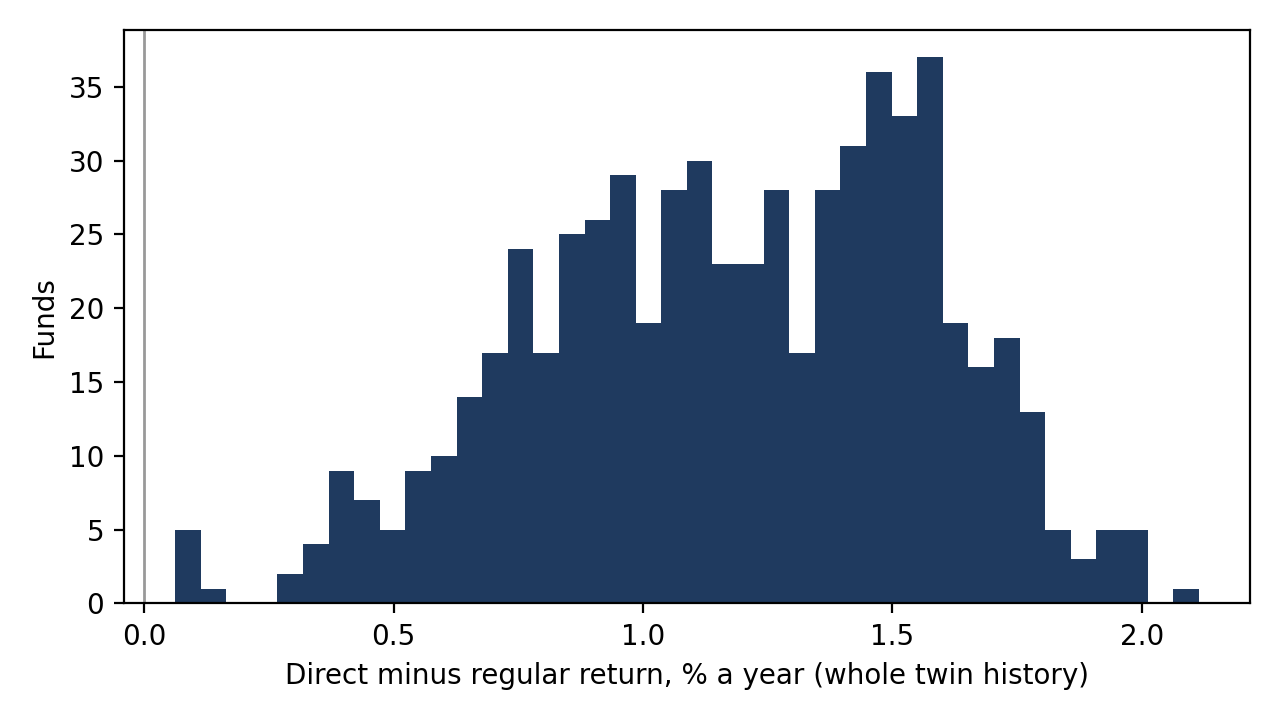
\includegraphics[width=0.49\linewidth]{commission_hist.png}\hfill
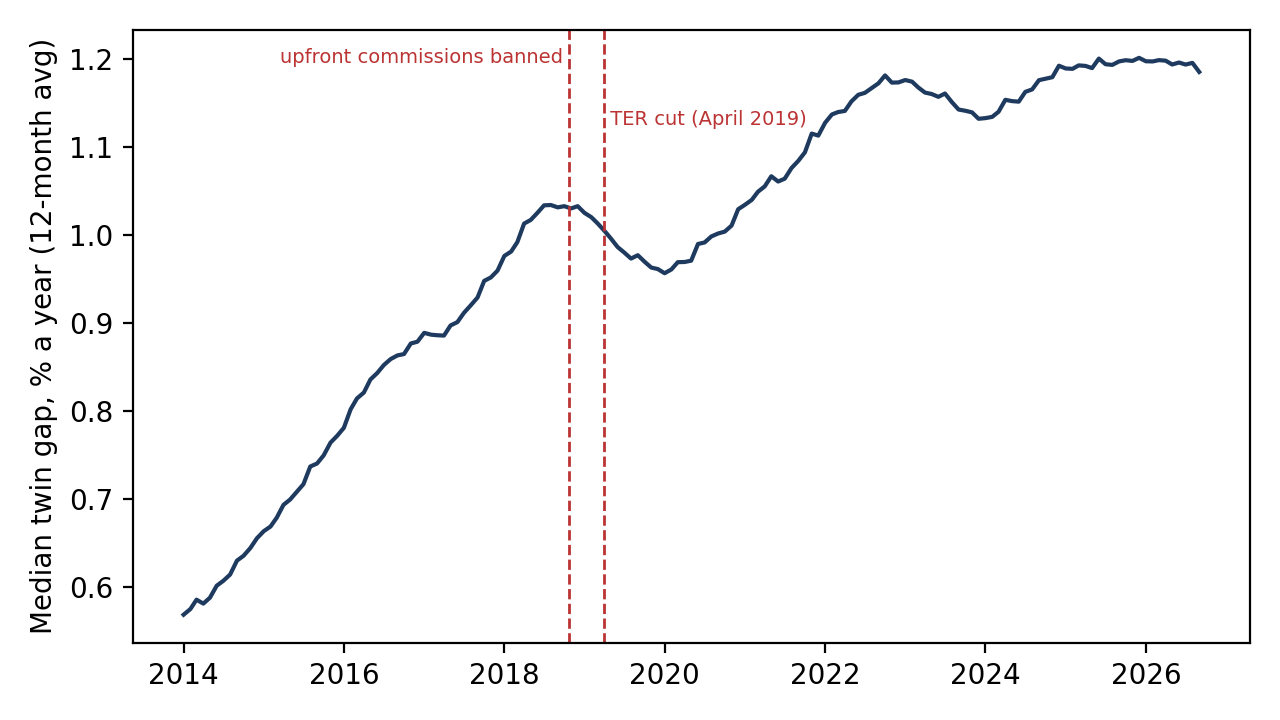
\includegraphics[width=0.49\linewidth]{commission_over_time.png}
\caption{Left: the direct-minus-regular gap of every twin pair over its whole history; none is below zero. Right: the median gap, 12-month average, with the two regulatory events.}\label{fig:comm}
\end{figure}

\begin{table}[htbp]\centering
\caption{The twin gap by category, \% a year.}\label{tab:commcat}
{\small\begin{tabular}{lrrr}
\toprule
Category & Twin pairs & Mean gap, \%/yr & Median gap, \%/yr \\
\midrule
Small Cap & 34 & 1.31 & 1.42 \\
Multi Cap & 36 & 1.35 & 1.41 \\
Sectoral/Thematic & 229 & 1.25 & 1.33 \\
Flexi Cap & 41 & 1.21 & 1.32 \\
Contra & 3 & 1.10 & 1.27 \\
Large \& Mid Cap & 35 & 1.19 & 1.22 \\
Mid Cap & 36 & 1.20 & 1.18 \\
Focused & 33 & 1.23 & 1.17 \\
Large Cap & 38 & 1.17 & 1.12 \\
Dividend Yield & 12 & 1.09 & 1.10 \\
ELSS & 51 & 1.09 & 1.09 \\
Value & 24 & 1.08 & 0.96 \\
Pre-2018 equity & 50 & 0.75 & 0.63 \\
\bottomrule
\end{tabular}
}
\end{table}

\begin{table}[htbp]\centering
\caption{Event tests: within-pair change in the annualised gap, 12 months after minus 12 months before.}\label{tab:events}
{\small\begin{tabular}{llrrrrr}
\toprule
Event date & Role & Pairs & Gap before & Gap after & Change & p (t-test) \\
\midrule
2019-04-01 & primary & 266 & 1.07 & 0.96 & -0.11 & <0.001 \\
2018-10-22 & secondary & 260 & 1.10 & 0.98 & -0.12 & <0.001 \\
2016-04-01 & placebo & 247 & 0.91 & 0.96 & 0.05 & 0.018 \\
2022-04-01 & placebo & 302 & 1.16 & 1.15 & -0.01 & 0.334 \\
\bottomrule
\end{tabular}
}
\end{table}

\section{Leak 2: skill, luck and the benchmark}\label{sec:skill}
\textbf{Is the yardstick fair?} If the four-factor model misprices Indian indices, every fund's alpha would carry the error. Index funds give a test: they should show about zero alpha. They do (Table~\ref{tab:calib}): Nifty 50 funds \CalibNiftyFiveZeroAlpha{} a year ($t$ = \CalibNiftyFiveZeroT) and Sensex funds \CalibSensexAlpha{} ($t$ = \CalibSensexT). The mid- and small-cap index series are too short to judge (\CalibMidcapOneFiveZeroMonths{} and \CalibSmallcapTwoFiveZeroMonths{} months; neither significant).

\textbf{How many funds have real skill?} Regular plans, the version most investors hold, earned a mean four-factor alpha of \SkillRegMeanAlpha{} a year after all fees (\SkillRegFunds{} diversified funds, 2006 to 2025); \SkillRegSharePosAlpha{} were positive. Many positive alphas are luck, so the Barras, Scaillet and Wermers (2010) false discovery method, with Newey and West (1987) $t$-statistics, per-fund bootstrap p-values (Kosowski et al.\ 2006) and Storey's (2002) estimate of the null share, estimates the shares of funds with truly zero, positive and negative alpha (Table~\ref{tab:fdr}). For regular plans, \SkillRegPiPlus{} have truly positive alpha (95\% interval \SkillRegPiPlusLo{} to \SkillRegPiPlusHi), \SkillRegPiZero{} have zero, and essentially none have negative alpha (upper bound \SkillRegPiMinusHi). Direct plans, closer to the manager's gross skill, do better: \SkillDirPiPlus{} have truly positive alpha (\SkillDirPiPlusLo{} to \SkillDirPiPlusHi). The registered hypothesis that fewer than 10\% of funds have positive alpha is rejected. Requiring 60 months of history gives the same picture (\SkillRegMinSixZeroPiPlus{} and \SkillDirMinSixZeroPiPlus).

\textbf{Do the best funds beat luck?} The Fama and French (2010) bootstrap builds a world in which every fund has zero true alpha and compares the actual distribution of $t$-statistics with it (Table~\ref{tab:ff}, Figure~\ref{fig:ff}). Above the 10th percentile, actual $t$-statistics beat the zero-alpha world in most simulations; at the 99th percentile the actual value of \SkillFfRegPNineNineT{} exceeds \SkillFfRegPNineNineShareBelow{} of simulations. At the bottom, the worst funds are no worse than bad luck.

\textbf{Against what an investor can actually buy.} Following Berk and van Binsbergen (2015), skill is also measured against alternatives an investor could hold. Against index funds (Sharpe 1992 style analysis on Nifty 50, Next 50, Midcap 150 and Smallcap 250 index funds, \StyleStart{} to \StyleEnd, \StyleMonths{} months, \StyleDirFunds{} funds), the median direct plan earned \StyleDirMedianAlpha{} a year and the median regular plan \StyleRegMedianAlpha. \StyleDirShareSigPos{} of direct plans but only \StyleRegShareSigPos{} of regular plans are significantly ahead. Against an investable benchmark, the commission eats most of the edge.

\textbf{Does skill persist?} Funds sorted each December on their prior 36-month alpha $t$-statistic (Carhart 1997) keep their order a year later (Table~\ref{tab:persist}): the top quintile earns \SkillPersistTopAlpha{} next year ($t$ = \SkillPersistTopT), the bottom \SkillPersistBottomAlpha, a spread of \SkillPersistSpreadAlpha{} ($t$ = \SkillPersistSpreadT).

\textbf{Discounting luck fund by fund.} An empirical-Bayes shrinkage pulls each fund's alpha toward the average, more when the estimate is noisy. The spread of true alphas across regular plans is \SkillRegEbTau{} a year, and \SkillRegEbShareProbNineZero{} of regular plans have at least a 90\% chance that their true alpha is positive. Out of sample (estimated 2013 to 2019, realised 2020 to 2025, \SkillDirOosFunds{} funds), shrinkage cut the prediction error (mean squared error \SkillDirOosMseRaw{} to \SkillDirOosMseShrunk) without changing the rank correlation (\SkillDirOosRhoRaw); but those funds' realised alpha averaged only \SkillDirOosMeanLaterAlpha{} (Section~\ref{sec:decay}).

\textbf{Survivorship matters.} Regular plans still alive earned \SkillRegAlphaAlive{} a year against \SkillRegAlphaDead{} for the \SkillRegDeadFunds{} that closed. A study of today's fund list would report an average alpha of \SkillRegAlphaAlive{} instead of \SkillRegAlphaAll{} for all regular plans.

\begin{table}[htbp]\centering
\caption{Calibration: index funds' own four-factor alpha.}\label{tab:calib}
{\small\begin{tabular}{llrrr}
\toprule
Index funds & Months used & Four-factor alpha, \%/yr & $t$ (NW) & $R^2$ \\
\midrule
Nifty Midcap 150 & 2021-03 to 2025-12 & 2.90 & 1.20 & 0.91 \\
Nifty Next 50 & 2010-07 to 2025-12 & -0.29 & -0.17 & 0.88 \\
Nifty 50 & 2006-05 to 2025-12 & 0.78 & 0.58 & 0.93 \\
Sensex & 2006-05 to 2025-12 & 1.10 & 0.76 & 0.91 \\
Nifty Smallcap 250 & 2020-11 to 2025-12 & -3.33 & -1.42 & 0.92 \\
\bottomrule
\end{tabular}
}
\end{table}

\begin{table}[htbp]\centering
\caption{Skill and luck by the false discovery method: estimated shares of funds with truly zero ($\hat\pi_0$), positive ($\hat\pi^+$) and negative ($\hat\pi^-$) alpha, \%, with bootstrap intervals.}\label{tab:fdr}
{\small\begin{tabular}{lrrrrrr}
\toprule
Sample & Funds & $\hat\pi_0$ & $\hat\pi^+$ & 95\% CI & $\hat\pi^-$ & 95\% CI \\
\midrule
regular diversified & 402 & 68.41 & 29.17 & [21.4, 36.6] & 0.00 & [0.0, 1.3] \\
direct diversified & 319 & 40.75 & 59.72 & [51.9, 66.8] & 0.00 & [0.0, 0.3] \\
regular sectoral/thematic & 122 & 68.85 & 33.61 & [21.1, 47.2] & 0.00 & [0.0, 2.7] \\
regular diversified, 60+ months & 318 & 74.21 & 26.73 & [19.2, 34.9] & 0.00 & [0.0, 0.0] \\
direct sectoral/thematic & 121 & 62.44 & 45.55 & [32.2, 58.5] & 0.00 & [0.0, 0.0] \\
direct diversified, 60+ months & 244 & 49.18 & 58.61 & [49.3, 67.3] & 0.00 & [0.0, 0.0] \\
\bottomrule
\end{tabular}
}
\end{table}

\begin{table}[htbp]\centering
\caption{Fama-French bootstrap, regular plans: actual $t(\alpha)$ at each percentile against a world where every fund's true alpha is zero.}\label{tab:ff}
{\small\begin{tabular}{rrrr}
\toprule
Percentile & Actual $t(\alpha)$ & Zero-alpha world & \% of simulations below actual \\
\midrule
1 & -2.22 & -2.13 & 40 \\
2 & -1.86 & -1.88 & 48 \\
5 & -1.44 & -1.49 & 52 \\
10 & -0.86 & -1.15 & 71 \\
20 & -0.36 & -0.74 & 78 \\
30 & 0.07 & -0.44 & 86 \\
40 & 0.35 & -0.20 & 87 \\
50 & 0.57 & 0.04 & 86 \\
60 & 0.91 & 0.27 & 91 \\
70 & 1.42 & 0.52 & 97 \\
80 & 1.79 & 0.81 & 98 \\
90 & 2.25 & 1.23 & 98 \\
95 & 2.67 & 1.58 & 98 \\
98 & 3.15 & 1.97 & 98 \\
99 & 3.47 & 2.24 & 98 \\
\bottomrule
\end{tabular}
}
\end{table}

\begin{figure}[htbp]\centering
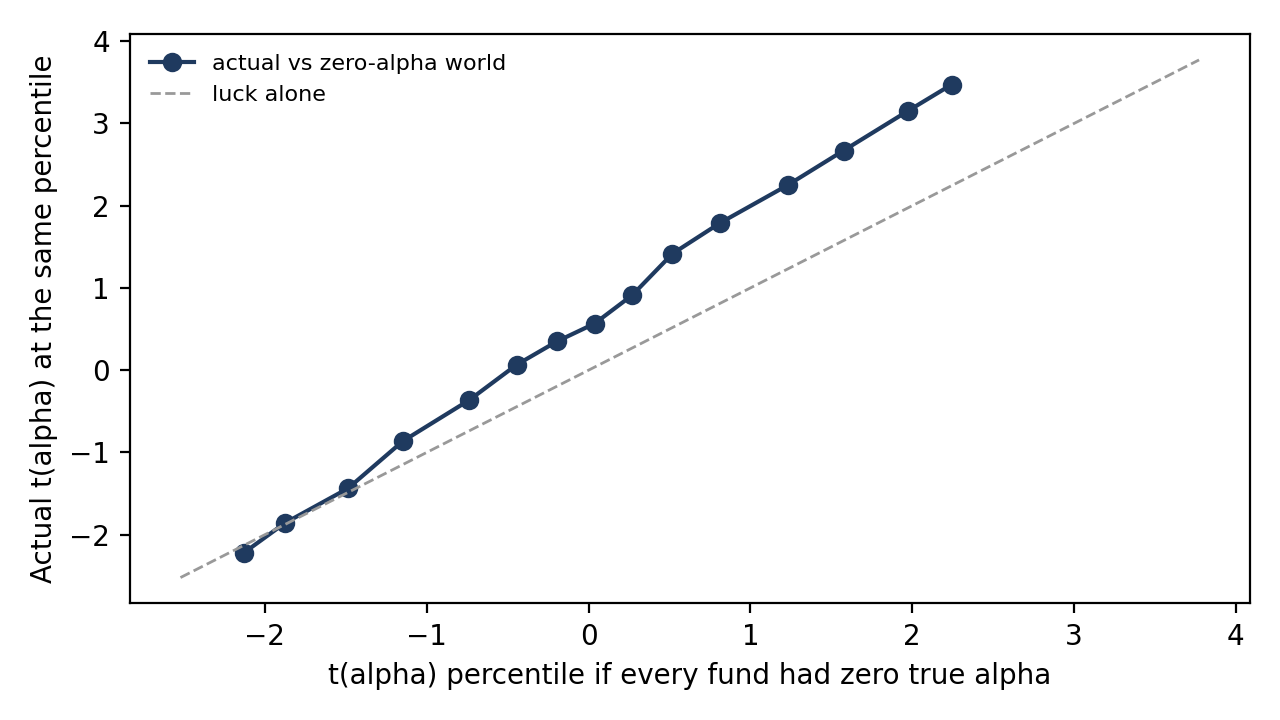
\includegraphics[width=0.62\linewidth]{skill_ff_bootstrap.png}
\caption{Actual $t(\alpha)$ percentiles against the zero-alpha world. Points above the dashed line are better than luck alone.}\label{fig:ff}
\end{figure}

\begin{table}[htbp]\centering
\caption{Persistence: next-year alpha of quintiles sorted on prior 36-month $t(\alpha)$.}\label{tab:persist}
{\small\begin{tabular}{lrrr}
\toprule
Portfolio (sorted on prior 36-month $t(\alpha)$) & Next-year alpha, \%/yr & $t$ (NW) & Months \\
\midrule
Quintile 1 & 0.68 & 0.62 & 192 \\
Quintile 2 & 1.05 & 0.86 & 192 \\
Quintile 3 & 1.58 & 1.39 & 192 \\
Quintile 4 & 2.52 & 2.15 & 192 \\
Quintile 5 & 3.36 & 2.71 & 192 \\
Top minus bottom & 2.67 & 3.61 & 192 \\
\bottomrule
\end{tabular}
}
\end{table}

\section{Leak 3: timing}
Across all active equity funds from \TimingStart{} to \TimingEnd{} (\TimingMonths{} months), the funds earned a time-weighted \TimingTwr{} a year and their investors a money-weighted \TimingMwr: a gap of \TimingGap{} (Table~\ref{tab:timing}). The time-weighted series built from AUM and flows tracks NAV-based category returns closely (correlation \TimingNavCorr).

\textbf{Is it bad timing?} The registered test places the same flows in random months, holding the return path fixed. Investors did worse than that (permuted gap \TimingVsRandom; $p$ \TimingPWorseRandom). But net inflows rose steeply over the period as SIP contributions grew (Rs \TimingTotalInflowCr{} in total, against average assets of Rs \TimingAvgAumCr), and shuffling across years moves today's large flows into early months that preceded the strongest returns. The added test, logged before results, shuffles flows only within each calendar year. Against it, investors' timing is no worse than random (\TimingVsRandomWithinYear; $p$ = \TimingPWorseRandomWithinYear). Flows also lean against recent returns: net flows as a share of assets fall after strong quarters (coefficient \TimingChasePastCoef, $t$ = \TimingChasePastT), the opposite of return-chasing. So most of the measured gap is money arriving later, after the best returns, not panic selling.

By category the gap is largest in small-cap funds (\TimingCatSmallCapGap) and absent in tax-saving ELSS funds (\TimingCatElssGap), whose flows follow the tax calendar and are locked in for three years.

\begin{table}[htbp]\centering
\caption{Time-weighted (funds) against money-weighted (investors) returns, \% a year, with the registered and the within-year permutation tests.}\label{tab:timing}
{\small\begin{tabular}{lrrrrr}
\toprule
Investors in & Funds (TWR) & Investors (MWR) & Gap & $p$ vs random & $p$ within-year \\
\midrule
All active equity & 14.93 & 14.28 & 0.65 & <0.001 & 0.199 \\
Large Cap Fund & 13.05 & 12.60 & 0.45 & 0.022 & 0.779 \\
Mid Cap Fund & 18.46 & 18.08 & 0.38 & <0.001 & 0.250 \\
Small Cap Fund & 19.93 & 18.89 & 1.05 & <0.001 & 0.050 \\
Large \& Mid Cap Fund & 15.81 & 14.89 & 0.92 & <0.001 & 0.373 \\
ELSS & 12.46 & 12.71 & -0.24 & 0.979 & 0.965 \\
\bottomrule
\end{tabular}
}
\end{table}

\begin{figure}[htbp]\centering
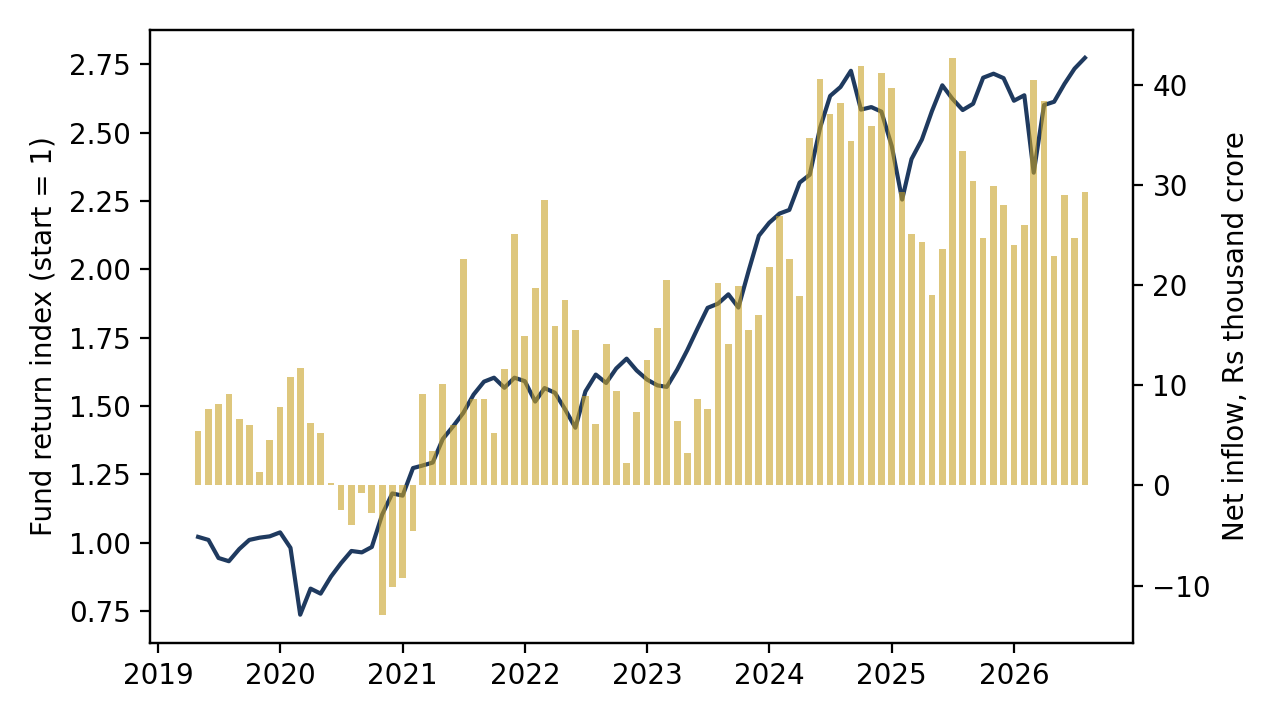
\includegraphics[width=0.62\linewidth]{timing_flows.png}
\caption{Active equity funds' return index (line) and monthly net inflows (bars). Flows grew most in the later years, after the steep gains of 2020 and 2021.}
\end{figure}

\section{Could the leaks have been avoided?}
Each December from 2013 to 2024, four registered rules picked funds using only information available on that day, held for a year: the lowest R-squared quintile (Amihud and Goyenko 2013), the highest prior-alpha quintile, ridge regression and gradient-boosted trees (Friedman 2001) trained on earlier years only (\SelFeatureRows{} fund-years of features). Out of sample (\SelYearsDirect), on direct plans (Table~\ref{tab:sel}, Figure~\ref{fig:sel}):
\begin{itemize}[leftmargin=1.2em]
\item The average active direct plan already earned \SelDirAllFundsAlpha{} a year of alpha ($t$ = \SelDirAllFundsT), against \SelDirNiftyFiveZeroIndexAlpha{} for Nifty 50 index funds ($t$ = \SelDirNiftyFiveZeroIndexT).
\item All four rules have significant alpha after the Holm (1979) correction, so the registered null is rejected. The trees did best: \SelDirGbtAlpha{} ($t$ = \SelDirGbtT, Holm $p$ = \SelDirGbtPholm).
\item What matters is the edge over simply holding every fund: trees \SelDirGbtVsall{} a year ($t$ = \SelDirGbtVsallT), high prior alpha \SelDirHighAlphaVsall{} ($t$ = \SelDirHighAlphaVsallT), ridge \SelDirRidgeVsall{} ($t$ = \SelDirRidgeVsallT), low R-squared \SelDirLowRTwoVsall{} ($t$ = \SelDirLowRTwoVsallT, not significant).
\item On regular plans the ranking holds (trees \SelRegGbtAlpha{} of alpha, \SelRegGbtVsall{} over all funds, $t$ = \SelRegGbtVsallT).
\end{itemize}
The edge was not stable over time. From 2014 to 2019 the trees beat all funds by \DecaySelGbtTwoZeroOneFourVsall{} ($t$ = \DecaySelGbtTwoZeroOneFourVsallT); from 2020 to 2025 by \DecaySelGbtTwoZeroTwoZeroVsall{} ($t$ = \DecaySelGbtTwoZeroTwoZeroVsallT). Only the high-prior-alpha rule stays significant in the later period (\DecaySelHighAlphaTwoZeroTwoZeroVsall, $t$ = \DecaySelHighAlphaTwoZeroTwoZeroVsallT).

\begin{table}[htbp]\centering
\caption{Out-of-sample fund selection, direct plans, \% a year.}\label{tab:sel}
{\small\begin{tabular}{lrrrrrr}
\toprule
Strategy (direct plans) & Excess return & Alpha & $t$ & Holm $p$ & Alpha vs all funds & $t$ \\
\midrule
Low $R^2$ quintile & 12.08 & 3.60 & 2.69 & 0.019 & 0.84 & 1.57 \\
High prior alpha quintile & 14.01 & 4.47 & 2.72 & 0.019 & 1.71 & 2.93 \\
Ridge regression & 13.30 & 4.30 & 2.69 & 0.019 & 1.54 & 2.08 \\
Gradient-boosted trees & 14.09 & 5.13 & 3.21 & 0.005 & 2.37 & 3.56 \\
All eligible funds & 11.45 & 2.76 & 1.99 &  &  &  \\
Nifty 50 index funds & 7.89 & 1.49 & 0.89 &  &  &  \\
\bottomrule
\end{tabular}
}
\end{table}

\begin{figure}[htbp]\centering
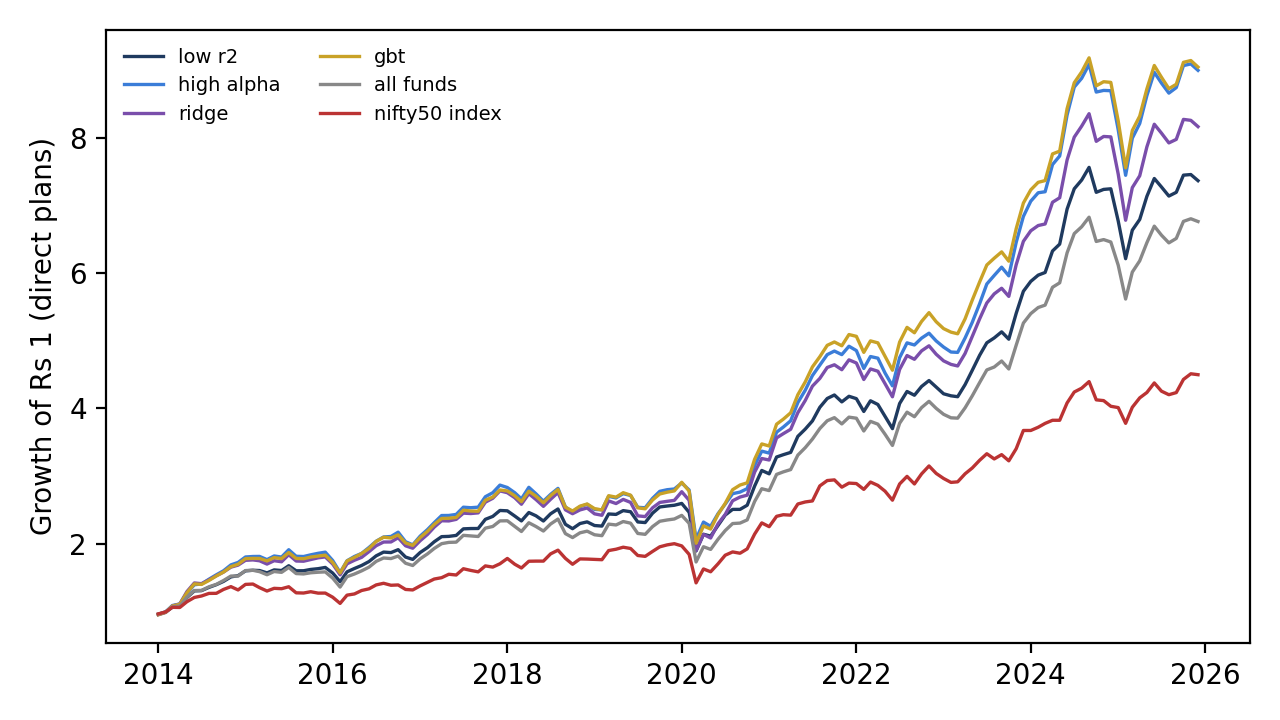
\includegraphics[width=0.62\linewidth]{selection_growth.png}
\caption{Growth of Rs 1 in each strategy's direct-plan picks, 2014 to 2025.}\label{fig:sel}
\end{figure}

\section{Exploratory: is the active edge fading?}\label{sec:decay}
This section was added after the main results (\texttt{DEVIATIONS.md}); it is exploratory. The rolling 36-month alpha of the average direct plan peaked at \DecayDirRollingMax{} in the window ending \DecayDirRollingMaxMonth, turned negative in 2022, and recovered to \DecayDirRollingLast{} in the latest window (Figure~\ref{fig:decay}). Year by year, with factor betas from the whole period, the average direct plan earned \DecayYearTwoZeroOneNineDir{} beyond the factors in 2019, \DecayYearTwoZeroTwoZeroDir{} in 2020, \DecayYearTwoZeroTwoOneDir{} in 2021, then \DecayYearTwoZeroTwoFourDir{} and \DecayYearTwoZeroTwoFiveDir{} in 2024 and 2025. Its alpha over 2013 to 2025 is \DecayDirAlphaFull{} ($t$ = \DecayDirAlphaFullT), and \DecayDirAlphaExTwoZeroTwoZero{} without 2020 ($t$ = \DecayDirAlphaExTwoZeroTwoZeroT).

The weaker period is also concentrated in older funds. Over 2020 to 2025, the \DecayOldFunds{} funds with three or more years of direct-plan history before 2020 earned \DecayOldAlpha{} a year, against \DecayNewAlpha{} for the \DecayNewFunds{} newer ones ($p$ \DecayOldnewP). This fits the idea that larger, older funds find it harder to beat the market, though age and size are not separated here. The realised alpha of \SkillDirOosMeanLaterAlpha{} in Section~\ref{sec:skill} is lower because that check also counts \DecayShortFunds{} older funds with only two to three years of data after 2019 (their series end between \DecayShortEndFirst{} and \DecayShortEndLast). Measured mostly on 2020 and 2021, they averaged \DecayShortAlpha{} a year; but the older funds that survived averaged \DecayOldwinAlpha{} over 2020 and 2021 as well, so the difference lies in the months covered, not in the funds.

\begin{figure}[htbp]\centering
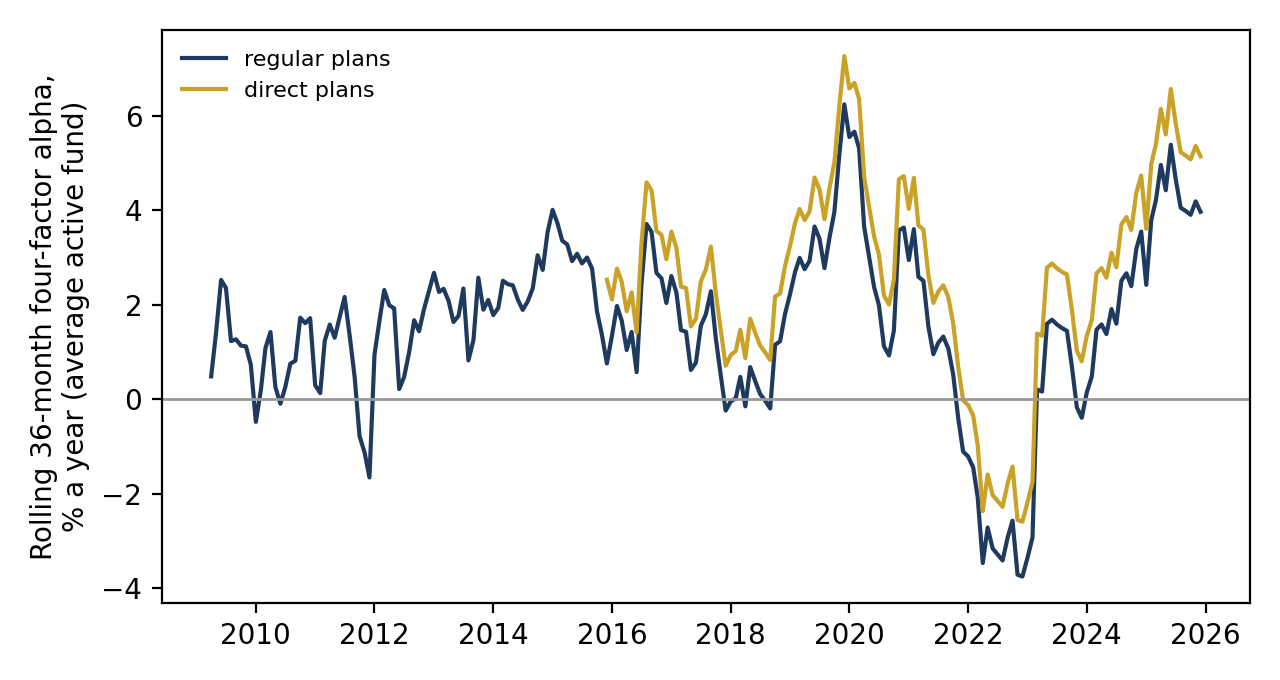
\includegraphics[width=0.62\linewidth]{decay_rolling_alpha.png}
\caption{Rolling 36-month four-factor alpha of the average active fund.}\label{fig:decay}
\end{figure}

\section{Exploratory: did SEBI's categorisation create closet index funds?}
SEBI's 2017 circular required large-cap funds to hold at least 80\% in the 100 largest stocks from mid-2018. If that squeezed out active bets, large-cap funds' tracking error against a Nifty 50 index fund should fall relative to mid- and small-cap funds, whose rules do not tie them to the largest stocks. It did not. Over the two years after mid-2018, large-cap funds' tracking error went from \ClosetAfterLargeTeBefore{} to \ClosetAfterLargeTePost{} a year (\ClosetAfterLargeN{} funds), mid- and small-cap funds' from \ClosetAfterControlTeBefore{} to \ClosetAfterControlTePost{} (\ClosetAfterControlN{} funds): a difference-in-differences of \ClosetAfterDidTe{} ($p$ = \ClosetAfterDidP), the opposite sign to closet indexing. A later window (2022 to 2024) gives \ClosetLaterDidTe{} ($p$ = \ClosetLaterDidP). This null is reported as found.

\section{The three leaks together}
On the one window where twin plans, consistent flow data and the factors all exist (\SynWindow, \SynMonths{} months), the leaks can be set side by side (Table~\ref{tab:syn}, Figure~\ref{fig:syn}). Direct plans returned \SynRetDirect{} a year, regular plans \SynRetRegular, the IIMA market portfolio (a fee-free benchmark of all listed Indian stocks) \SynRetMarket{} and Nifty 50 index funds \SynRetNiftyFiveZero.
\begin{itemize}[leftmargin=1.2em]
\item \textbf{Skill} was a gain, not a leak: direct plans beat the market portfolio, so the skill leak is negative, \SynSkillVsMarket{} a year (Rs \SynRsSkillCr{} at 2025 assets). Measured against Nifty 50 index funds it is \SynSkillVsNiftyFiveZero, mostly because mid- and small-cap stocks beat large caps in this window, which is style, not skill.
\item \textbf{Commission} cost \SynCommission{} a year, Rs \SynRsCommissionCr.
\item \textbf{Timing} cost \SynTiming{} a year on this window, Rs \SynRsTimingCr, mostly the late arrival of money rather than bad month-to-month timing.
\end{itemize}
The pieces are measured on their natural bases (equal-weighted funds for skill and commission, AUM for timing), so they add up only approximately.

\begin{table}[htbp]\centering
\caption{The three leaks on one window, points a year and Rs crore a year at 2025 assets. Negative means a gain to investors.}\label{tab:syn}
{\small\begin{tabular}{lrr}
\toprule
Leak (2019-05 to 2025-12) & Points a year & Rs crore a year at 2025 AUM \\
\midrule
Skill (passive market minus direct plans) & -0.49 & -15,852 \\
Commission (direct minus regular twins) & 1.25 & 31,906 \\
Timing (funds' TWR minus investors' MWR) & 0.29 & 9,243 \\
\bottomrule
\end{tabular}
}
\end{table}

\begin{figure}[htbp]\centering
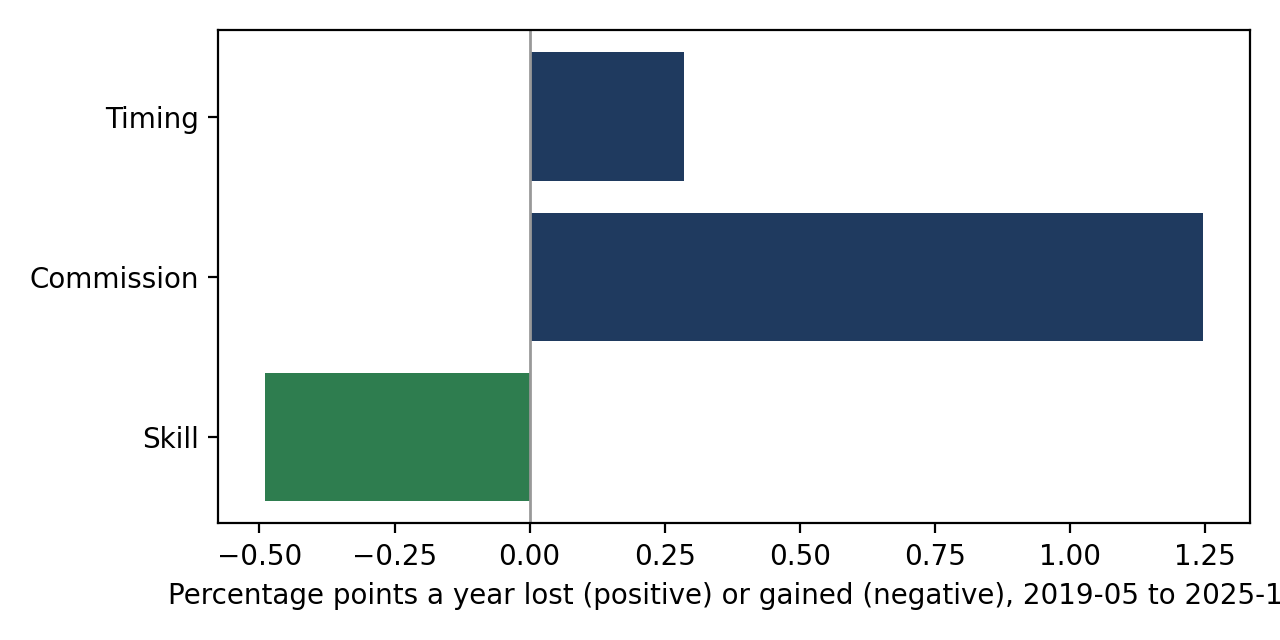
\includegraphics[width=0.62\linewidth]{synthesis_leaks.png}
\caption{The three leaks, \SynWindow.}\label{fig:syn}
\end{figure}

\section{Deployment}
\paragraph{The scorecard.} \texttt{docs/index.html} is a single offline page covering all \CardFunds{} live active equity funds with both plans. For each it shows the yearly cost of the regular plan over the last 36 months (median \CardCommissionMedian, one in ten above \CardCommissionPNineZero), the direct plan's alpha with its false-discovery $q$-value, the empirical-Bayes expected alpha and the chance it is positive, R-squared, a verdict and the cheaper index alternative. The verdict rule was fixed before any fund's result was read: $q \le 0.10$ with a positive $t$ is ``evidence of skill'', with a negative $t$ ``evidence of underperformance'', otherwise ``indistinguishable from luck''. Of the funds, \CardSkill{} show evidence of skill, \CardUnder{} show evidence of underperformance and \CardLuck{} are indistinguishable from luck; \CardSector{} sector funds get no verdict, because the market factors are not their benchmark, and \CardShort{} have too little history.

\paragraph{What it means for investors and platforms.} Choosing the direct plan of the same fund is the one free improvement available to every investor, worth about \CardCommissionMedian{} a year at the median. Fund selection on past evidence helped, but by less after 2019, so the scorecard shows uncertainty (the $q$-value and the chance of positive alpha), not rankings.

\paragraph{Disclosure ideas for SEBI.} Show each regular plan's realised return gap to its direct twin, in rupees on the investor's own holding, on every account statement; and publish both plans' returns side by side in every factsheet.

\section{Limitations}
\begin{itemize}[leftmargin=1.2em]
\item Regular plans' share of equity assets is borrowed from AMFI's figure for SIP assets, so the rupee estimates carry that assumption (hence the range).
\item The four-factor model is fair for large-cap indices; the mid- and small-cap index series are too short to confirm it there. Investable-benchmark results cover only 2021 onwards.
\item Scheme-wise AUM is not published at a fixed address, so funds are equal-weighted; timing is measured on AMFI's aggregates, not individual accounts.
\item The selection results hold for this period and these rules; the edge weakened after 2019.
\item The decay and closet-indexing sections are exploratory and were not pre-registered.
\end{itemize}

\section{Reproducibility}
Every number in this report is written by the pipeline into \nolinkurl{results/numbers.json} and \nolinkurl{report/numbers.tex}; none is typed by hand. \texttt{make all} downloads the raw data from AMFI and IIMA, rebuilds every panel, reruns every analysis with fixed random seeds, and recompiles this report. A full rerun from the downloaded files reproduces every number exactly. Raw data is not redistributed; the download scripts fetch it from the publishers.

\section*{References}
\begin{small}
\begin{itemize}[leftmargin=1em,label={}]
\item Agarwalla, S. K., Jacob, J. and Varma, J. R. (2013). Four factor model in Indian equities market. IIMA Working Paper 2013-09-05.
\item AMFI and Crisil (2025). \textit{AMFI Annual Report FY 2025}. Association of Mutual Funds in India.
\item Amihud, Y. and Goyenko, R. (2013). Mutual fund's $R^2$ as predictor of performance. \textit{Review of Financial Studies} 26(3).
\item Barras, L., Scaillet, O. and Wermers, R. (2010). False discoveries in mutual fund performance: measuring luck in estimated alphas. \textit{Journal of Finance} 65(1).
\item Bergstresser, D., Chalmers, J. and Tufano, P. (2009). Assessing the costs and benefits of brokers in the mutual fund industry. \textit{Review of Financial Studies} 22(10).
\item Berk, J. B. and van Binsbergen, J. H. (2015). Measuring skill in the mutual fund industry. \textit{Journal of Financial Economics} 118(1).
\item Carhart, M. M. (1997). On persistence in mutual fund performance. \textit{Journal of Finance} 52(1).
\item DeMiguel, V., Gil-Bazo, J., Nogales, F. J. and Santos, A. A. P. (2023). Machine learning and fund characteristics help to select mutual funds with positive alpha. \textit{Journal of Financial Economics} 150(3).
\item Dichev, I. D. (2007). What are stock investors' actual historical returns? \textit{American Economic Review} 97(1).
\item Fama, E. F. and French, K. R. (2010). Luck versus skill in the cross-section of mutual fund returns. \textit{Journal of Finance} 65(5).
\item Friedman, J. H. (2001). Greedy function approximation: a gradient boosting machine. \textit{Annals of Statistics} 29(5).
\item Friesen, G. C. and Sapp, T. R. A. (2007). Mutual fund flows and investor returns: an empirical examination of fund investor timing ability. \textit{Journal of Banking and Finance} 31(9).
\item Holm, S. (1979). A simple sequentially rejective multiple test procedure. \textit{Scandinavian Journal of Statistics} 6(2).
\item Kosowski, R., Timmermann, A., Wermers, R. and White, H. (2006). Can mutual fund ``stars'' really pick stocks? \textit{Journal of Finance} 61(6).
\item Newey, W. K. and West, K. D. (1987). A simple, positive semi-definite, heteroskedasticity and autocorrelation consistent covariance matrix. \textit{Econometrica} 55(3).
\item Sharpe, W. F. (1992). Asset allocation: management style and performance measurement. \textit{Journal of Portfolio Management} 18(2).
\item Storey, J. D. (2002). A direct approach to false discovery rates. \textit{Journal of the Royal Statistical Society, Series B} 64(3).
\end{itemize}
\end{small}
\end{document}
